\documentclass[rnd]{mas_proposal}
% \documentclass[thesis]{mas_proposal}

\usepackage[utf8]{inputenc}
\usepackage{amsmath}
\usepackage{amsfonts}
\usepackage{amssymb}
\usepackage{graphicx}
\usepackage{listings}
\usepackage{xcolor}
\usepackage[edges]{forest}


\lstset{
  basicstyle=\ttfamily\small,
  breaklines=true,
  frame=single,
  backgroundcolor=\color{gray!10},
  keywordstyle=\color{blue}\bfseries,
}


\title{Shadow Casting Object Segmentation}
\author{Kai Glasenapp \\ Sai Mukkundan Ramamoorthy \\ Shrikar Nakhye}
\supervisors{Prof. Dr. Sebastian Houben}
\date{September 2025}

% \thirdpartylogo{path/to/your/image}

\begin{document}
\maketitle 
\pagestyle{plain}

\section{Introduction}

Semantic segmentation in aerial imagery is a critical task for smart city planning, 
urban monitoring, and emergency response. This project explores the segmentation 
of shadow-casting objects (e.g., buildings, trees) from aerial RGB images, focusing 
on the trade-off between segmentation accuracy and computational efficiency. 

The work was carried out in the context of the Hackathon about Segmentation of Aerial Images / Satellite Images by City of Bonn, 
with the aim of producing a lightweight segmentation pipeline that can operate under real-world time and hardware constraints. 

\section{Objectives}

\begin{itemize}
    \item Evaluate deep learning segmentation models (U-Net, Mask-RCNN).  
    \item Optimize models for speed and efficiency while maintaining accuracy.  
    \item Perform inference on real aerial images of Bonn City.  
    \item Benchmark models with metrics: IoU, F1, inference time, GPU memory usage.  
\end{itemize}

\section{Dataset}

The dataset consists of high-resolution aerial imagery provided by the City of Bonn (2024).  
Originally captured with an \textit{IGI UrbanMapper-2} camera at 2.5 cm/pixel resolution,  
the data was downsampled to 10 cm/pixel to comply with privacy regulations.  
The downsampled dataset (RGB only) is reduced to approximately 70 GB,  
allowing efficient training and inference on mid-range GPUs.  

Preprocessing steps included:
\begin{itemize}
    \item Cropping into smaller patches for training.  
    \item Removal of NIR channel.  
    \item Integration of hackathon crowd-sourced annotations.  
\end{itemize}

\section{Hardware and Environment}
\begin{itemize}
    \item OS: Linux (Kernel 6.8.0)  
    \item CPU: Intel Core i5-12400 (6 cores, 12 threads)  
    \item GPU: NVIDIA GeForce RTX 4070 (16 GB, CUDA 12.5)  
    \item Frameworks: PyTorch
\end{itemize}

\section{Methodology}

\section{Model Architectures}
\begin{itemize}
    \item \textbf{U-Net:} A classical encoder-decoder segmentation architecture originally designed for biomedical image segmentation \cite{unet}. 
    It consists of a contracting path (encoder) that captures context by progressively downsampling the input, 
    and an expansive path (decoder) that enables precise localization through upsampling and concatenation with 
    high-resolution features from the encoder (skip connections). These skip connections allow U-Net to 
    combine semantic information (from deep layers) with fine-grained spatial details (from shallow layers), 
    making it highly effective for pixel-level prediction tasks. 

    \textit{\textbf{Why U-Net for this task?}}  
    \begin{itemize}
        \item Performs well with limited training data due to efficient use of context and localization. 
        \item Skip connections preserve fine spatial details, crucial for distinguishing small or thin structures. 
        \item Lightweight compared to more complex models, enabling faster training and inference. 
        \item Proven strong performance across domains, making it a reliable baseline for remote sensing and 3D vision tasks. 
    \end{itemize}

    \item \textbf{Mask R-CNN:} A region-based convolutional neural network for instance segmentation, 
    extending Faster R-CNN by adding a parallel mask prediction branch. 
    Widely used for object-level precision in computer vision tasks such as autonomous driving and aerial imagery analysis.  

\end{itemize}


\subsection{Training Strategy: U-Net}
\begin{itemize}
    \item \textbf{Loss Function:} Cross-Entropy Loss.  
    \begin{itemize}
        \item Suitable for multi-class segmentation (foreground vs. background). 
        \item Penalizes pixel-level misclassification and provides stable gradients. 
        \item Efficient and supported in PyTorch. 
    \end{itemize}

    \item \textbf{Training Approach:} 
    \begin{itemize}
        \item Dataset split: 80\% training, 20\% validation using \texttt{train\_test\_split}. 
        \item Parameters updated via backpropagation with Adam optimization. 
        \item Validation monitored with IoU and F1-score. 
        \item Metrics and system resource usage logged for reproducibility. 
        \item Training for 20 epochs (balanced cost vs. convergence). 
    \end{itemize}

    \item \textbf{Evaluation Metrics During Training:} 
    \begin{itemize}
        \item Intersection over Union (IoU). 
        \item F1-score (precision-recall balance). 
    \end{itemize}

    \item \textbf{Hyperparameters:} 
    \begin{itemize}
        \item Learning Rate: $1 \times 10^{-4}$  
        \item Optimizer: Adam  
        \item Batch Size: 4  
        \item Number of Epochs: 20  
        \item Image Size: $512 \times 512$  
        \item Encoder Backbone: ResNet-34 pre-trained on ImageNet  
    \end{itemize}

    \item \textbf{Why This Strategy?}  
    \begin{itemize}
        \item Balances stability (small LR, Adam) with speed (transfer learning). 
        \item Cross-Entropy provides a strong baseline. 
        \item IoU and F1 ensure segmentation quality is captured beyond pixel accuracy. 
        \item Hyperparameters tuned for limited GPU memory. 
    \end{itemize}
\end{itemize}


\subsection{Training Strategy: Mask R-CNN (Placeholder)}
\textit{[Add details about Mask R-CNN loss functions, backbone, training schedule, and evaluation metrics.]}

\subsection{Evaluation Metrics}
To ensure fair and comprehensive comparison across different models, 
the following evaluation metrics were considered:
\begin{itemize}
    \item \textbf{Intersection over Union (IoU):} Measures the overlap between predicted and ground-truth segmentation masks.  
    \item \textbf{F1 Score:} Balances precision and recall, useful when classes are imbalanced.  
    \item \textbf{Inference Time:} Average time taken to process one image (ms per image).  
    \item \textbf{Training Time:} Total time required for training (measured in hours).  
    \item \textbf{GPU Memory Usage:} Peak VRAM consumption during training and inference.  
\end{itemize}

\section{Results and Discussion}

\subsection{Quantitative Results}
Table~\ref{tab:results} summarizes the benchmark results.

\begin{table}[h]
\centering
\begin{tabular}{lcccc}
\hline
\textbf{Model} & \textbf{IoU} & \textbf{F1} & \textbf{Inference (ms)} & \textbf{VRAM (GB)} \\
\hline
YOLOv8-seg & XX & XX & XX & XX \\
U-Net & 0.742 & 0.841 & 52 & 5.65 \\
Mask-RCNN & XX & XX & XX & XX \\
\hline
\end{tabular}
\caption{Comparison of models}
\label{tab:results}
\end{table}


\subsection{Qualitative Results}
Figure~\ref{fig:training_metrics} shows the training curves for U-Net, illustrating the decrease in training loss 
and the corresponding improvement in validation IoU and F1-score over 20 epochs.  

\begin{figure}[h]
\centering
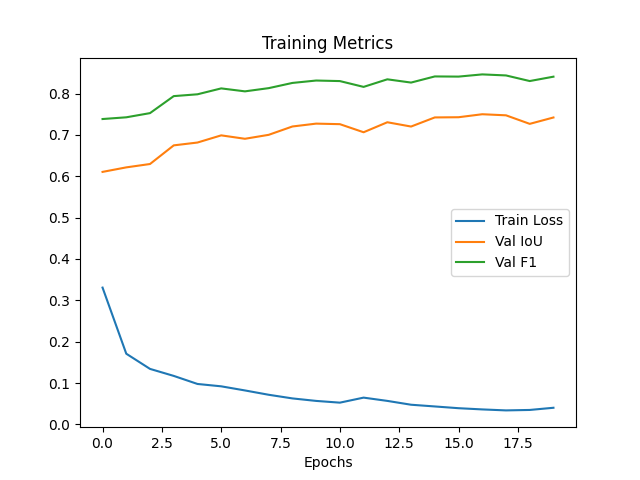
\includegraphics[width=0.7\textwidth]{images/training_metrics.png}
\caption{U-Net Training Metrics}
\label{fig:training_metrics}
\end{figure}

Figure~\ref{fig:segmentation} shows example segmentation outputs for U-Net compared to other models (placeholders).  

\begin{figure}[h]
\centering
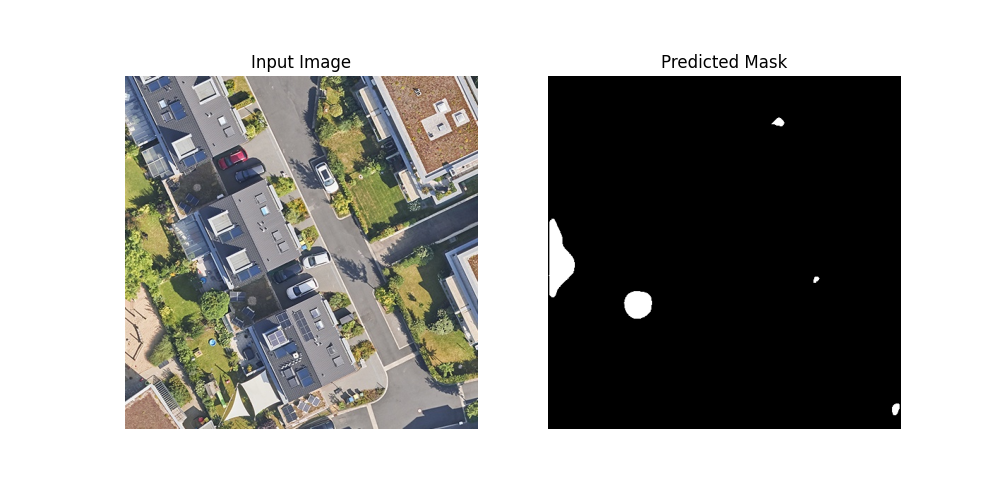
\includegraphics[width=0.9\textwidth]{images/inference_unet.png}
\caption{Example segmentation masks U-Net}
\label{fig:segmentation}
\end{figure}


\subsection{Discussion}
\begin{itemize}
    \item \textbf{U-Net:}  
    U-Net achieved a validation IoU of 0.742 and F1-score of 0.841, demonstrating strong pixel-level segmentation performance. 
    The model converged steadily within 20 epochs, with training loss decreasing from 0.33 to 0.04 and validation metrics stabilizing around epoch 15. 
    Inference was efficient at approximately 52 ms per image, with a VRAM footprint of 5.65 GB on the RTX 4050 Laptop GPU.  
    This indicates that U-Net provides a solid balance between performance and computational resource usage.

    \item \textbf{Mask R-CNN:}  
    \textit{[Add results and discussion once trained; typically excels in instance-level precision but may be slower and use more VRAM than U-Net.]}

    
    \item \textbf{Challenges:}  
    Despite good performance, shadow occlusion and variable sunlight conditions remain challenging for all models. 
    Fine-tuning data augmentation and loss functions may further improve robustness.
\end{itemize}
\newpage
\section{Documentation and Reproducibility}

\subsection{Minimum Working Example}

\begin{lstlisting}[language=bash,caption={Running PrithviVision},label={lst:mwe}]
git clone https://github.com/ItsShriks/Shadow_Casting_Object_Segmentation.git
cd PrithviVision
conda env create -f Essentials/dlrv.yml

conda activate dlrv


# Training
python src/train_unet.py -h

# Inference
python inference_unet.py -h
\end{lstlisting}

\subsection{Repository Structure}\cite{PrithviVision2025}
\begin{forest}
for tree={
    font=\ttfamily,
    grow'=0,
    child anchor=west,
    parent anchor=south,
    anchor=west,
    calign=first,
    inner xsep=7pt,
    edge path={
        \noexpand\path [draw, \forestoption{edge}]
        (!u.south west) ++(3pt,0) |- (.child anchor) \forestoption{edge label};
    },
    before typesetting nodes={
        if n=1
            {insert before={[,phantom]}}
            {}
    },
    fit=band,
    before computing xy={l=15pt},
}
[PrithviVision/
  [Essentials/ \quad {\small (environment \& setup files)}
    [dlrv.yml \quad {\small (Conda environment file)}]
  ]
  [Proposal/ \quad {\small (project proposal documents)}]
  [dataset/ \quad {\small (training/validation data)}
    [unet\_dataset/ \quad {\small (for U-Net segmentation)}
      [images/ \quad {\small (input images)}]
      [masks/ \quad {\small (ground truth masks)}]
    ]
    [yolo\_dataset/ \quad {\small (for YOLO object detection)}
      [train/ \quad {\small (training images \& labels)}]
      [valid/ \quad {\small (validation images \& labels)}]
    ]
  ]
  [outputs/ plots/ \quad {\small (results, segmentation outputs)}]
  [src/ \quad {\small (source code)}
    [train\_unet.py \quad {\small (U-Net training script)}]
    [inference\_unet.py \quad {\small (U-Net inference script)}]
  ]
  [.gitignore \quad {\small (Git ignore configuration)}]
  [README.md \quad {\small (project overview \& usage guide)}]
]
\end{forest}

\section{Conclusion and Future Work}


Future directions for this research include:
\begin{itemize}
    \item Applying model quantization and optimization for efficient deployment on edge devices such as NVIDIA Jetson.  
    \item Expanding to larger and more diverse datasets to improve robustness and generalization across different environments.  
\end{itemize}

\nocite{*}
\bibliographystyle{plainnat}
\bibliography{bibliography.bib}

\end{document}
